\documentclass[11pt]{scrartcl}

% standard packages
\usepackage[utf8]{inputenc}  % input in UTF-8
\usepackage[T1]{fontenc}  % output in T1 fonts (westeuropäische Codierung)
\usepackage{lmodern}  % latin modern fonts
\usepackage[ngerman]{babel}  % deutsches Sprachpaket, neue Rechtschreibung

% Seitensetup
\usepackage{scrlayer-scrpage}  % Seitenformatierung durch KOMA-interne Optionen
\usepackage[top=4cm, bottom=4cm]{geometry}  % Seitengeometrie (kann durch KOMA ersetzt werden, hab ich aber nicht geschafft)
\usepackage[hypcap=false]{caption, subcaption}  % caption editing - hypcap warning with hyperref
\usepackage{array}  % table editing

% additional packages
\usepackage{amsmath, amssymb, amstext}  % math packages (American Math Society)
\usepackage{bm}
\usepackage{icomma}  % Kommata in Dezimalzahlen verursachen keinen Abstand mehr
\usepackage{graphicx}  % Bilder einfügen
\usepackage{float} %Bilder placement
\usepackage{pdfpages}  % PDF als vollständige Seiten einfügen
\usepackage{lastpage}  % referenziert die letzte Seite
\usepackage[separate-uncertainty=true]{siunitx}  % bessere Darstellung von Einheiten
\usepackage{makecell} %Dicke Tabellenstriche
\usepackage{longtable}
\usepackage{booktabs}
%\usepackage{datatool}
\usepackage[hidelinks]{hyperref}  % hyperref verlinkt Referenzen - hidelinks entfernt borders um links

% package setups
% Kopf- und Fußzeile durch KOMA
\pagestyle{scrheadings}  % KOMA darf entscheiden
\clearpairofpagestyles  % reset
\setkomafont{pageheadfoot}{\normalfont}  % Standardschrift in Kopf- und Fußzeile
\captionsetup{format=plain, font=small, labelfont=bf} %Better caption, Abbildung ist FETT
%\setlength{\headheight}{27.2pt}  % benötigte Höhe Kopfzeile (warning von scrlayer-scrpage, wird aber automatisch so gerendert, falls diese Option weggelassen wird)
\ihead{Quincke Kundt}  % Kopf links %Todo Titel ändern
\chead{\textsc{Philipp} Maximilian}  % Kopf Mitte %Todo Name ändern
\ohead{16 Mai 2021}  % Kopf rechts %Todo Datum ändern
\cfoot{\pagemark \, / \pageref{LastPage}}  % Fuß Mitte

% Table of Contents
\DeclareTOCStyleEntry{dottedtocline}{section}  % KOMA intern - Inhaltsverzeichnis mit Punkten (nur sections)

%Overbar setup
\newcommand{\overbar}[1]{\mkern 1.5mu\overline{\mkern-1.5mu#1\mkern-1.5mu}\mkern 1.5mu}
% SI
\sisetup{locale = DE}  % deutschsprachige SI-Konvention
\sisetup{quotient-mode = fraction}
\sisetup{per-mode = fraction}
\DeclareSIUnit\px{px}

% citation
\usepackage{csquotes}
\usepackage[backend=biber]{biblatex}
\addbibresource{quincke-kundt.bib} %Todo .bib befüllen zb.: mit JabRef (Empfehlung der Redaktion)

% array
\renewcommand{\arraystretch}{1.2}

\begin{document}

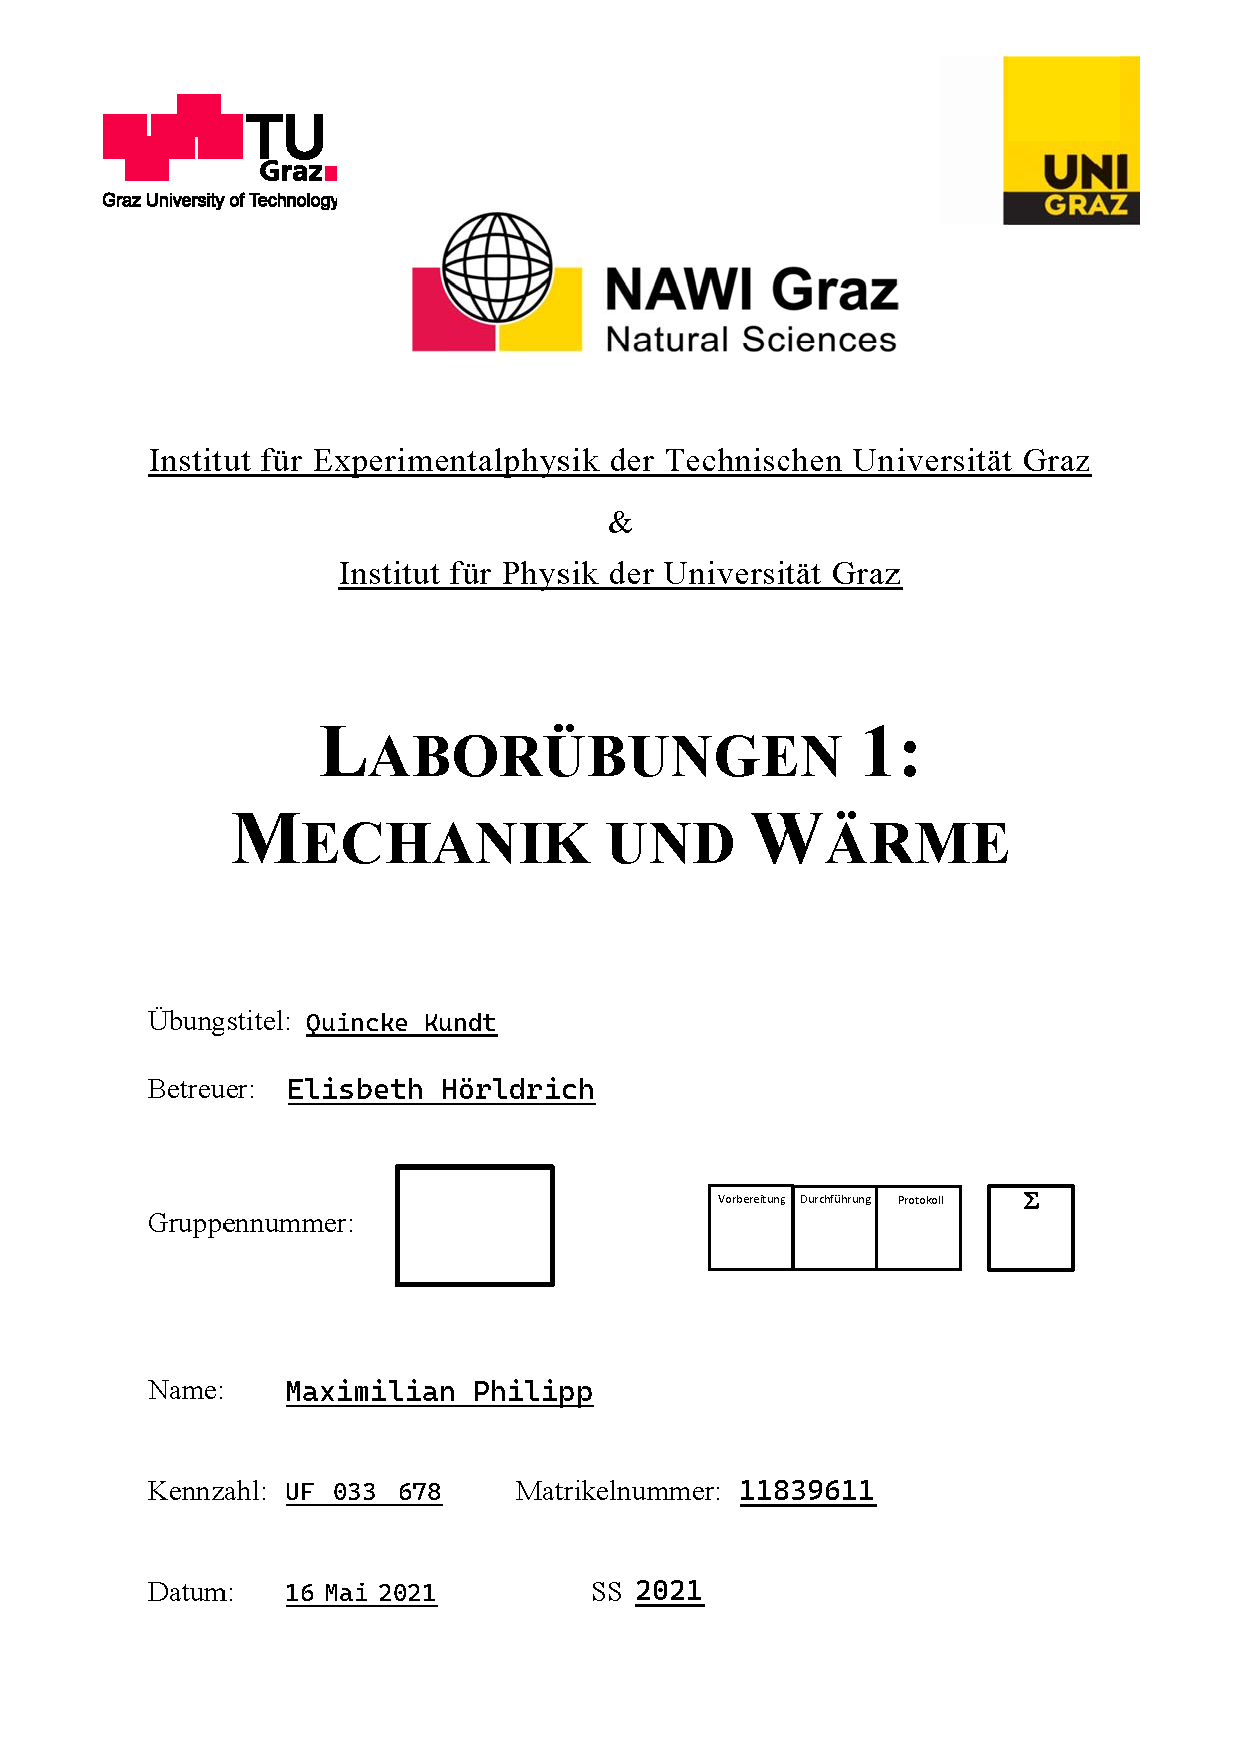
\includepdf{pdfs/Deckblatt.pdf} % Todo Deckblatt ausfüllen

\tableofcontents
\newpage
\section{Aufgabenstellung}
\label{sec:aufgabenstellung}

Die folgenden Punkte sind zu erfüllen:
\begin{enumerate}
    \item Bestimmung der Schwingungsknoten der stehenden Welle im Quincke-Resonanzrohr.
    \item Bestimmung der Schallgeschwindigkeit in Luft.
    \item Berechnung des Adiabatenexponenten von Luft.
    \item Bestimmung der Wellenlänge einer stehenden Welle (5 Messungen) im Kundt’schen Rohr.
    \item Berechnung des Elastizizätsmoduls des Stabes unter Verwendung der mit dem Quincke-Resonanzrohr bestimmten Schallgeschwindigkeit in Luft.
\end{enumerate}

\section{Voraussetzungen und Grundlagen}
\label{sec:voraussetzungen_grundlagen}

Der Schall breitet sich in Gasen als longitudinale Welle aus, d.h. 
die Teilchen schwingen in
Ausbreitungsrichtung der Welle. In zwei Medien gilt mit $\nu$
der Frequenz, mit $\lambda, \lambda'$ und $c, c'$ den
jeweiligen Wellenlängen und Schallgeschwindigkeiten:

\begin{equation}
    \label{eq:cist}
    c = \lambda \nu \qquad \text{und} \qquad c' = \lambda' \nu
\end{equation}

Wird Schall reflektiert, so bilden, bei geeigneten Bedingungen, 
die mit der einfallenden interferierende
reflektierte Welle eine stehende Welle. Für Reflexion am einen offenen 
Ende und
am anderen starren Ende (Wasseroberfläche) gilt die Resonanzbedingung, 
daß die Länge der
Luftsäule ein ungeradzahliges Vielfaches eines Viertels der Wellenlänge
sein muß.

\begin{equation}
    l_{1} = \frac{1}{4} \lambda,\; l_{2} = \frac{3}{4} \lambda,\;  l_{3} = \frac{5}{4} \lambda,\;  \cdots,\;  l_{n} = \frac{2n-1}{4} \lambda \qquad n = 1,2,3, \dots  \label{eq:lambda_avg}
\end{equation}

Der temperaturabhängige Quotient des Drucks $p$ und 
der Dichte $\rho$ steht mit $p_0$ (1013 mbar)
und $\rho_0$ (\SI{1.29e-3}{\gram\per\cm\cubed}), dem Luftdruck und -dichte 
bei \SI{0}{\celsius} auf Meereshöhe, und  dem
Spannungskoeffizienten der Luft ($\alpha=$\SI{1/273.15}{\per\kelvin}) 
im Zusammenhang:

\begin{equation}
    \frac{p}{\rho}=\frac{p_0}{\rho_0}(1+\alpha \theta)
\end{equation}

Damit ergibt sich aus der Schallgeschwindigkeit $c$ nach Laplace für 
die von der Temperatur
abhängige Schallgeschwindigkeit $c_T$:

\begin{equation}
    c = \sqrt{\frac{p\kappa}{\rho}} \qquad \implies \qquad c_T = \sqrt{\frac{p_0\kappa(1+\alpha \theta)}{\rho_0}} \label{eq:kappa_c}
\end{equation}

Für Luft gilt näherungsweise im Temperaturbereich \SI{-20}{\celsius} 
$\Rightarrow$ \SI{40}{\celsius} die Zahlenwertgleichung:

\begin{equation}
    c \; [\si{\meter\per\second}] = 331,5 + 0,6 \; \theta \; [\si{\celsius}] 
\end{equation}

Beim Übergang von einem Medium ins andere gibt sich nach \autoref{eq:cist}

\begin{equation}
    \frac{c}{c'}=\frac{\lambda}{\lambda'} \label{eq:wellenlangen_verhaltnis}
\end{equation}


d.h. in zwei verschiedenen Medien verhalten sich die 
Ausbreitungsgeschwindigkeiten einer Welle wie ihre Wellenlängen.
Die Frequenz ändert sich dabei nicht. Wird also die Wellenlänge in
beiden Medien gemessen, und ist die Schallgeschwindigkeit in einem Medium 
bekannt, so ist die Schallgeschwindigkeit im anderen Medium aus 
\autoref{eq:wellenlangen_verhaltnis} bestimmbar.
Bei bekannter Dichte des Stabmaterials (Dichte von Glas bei Raumtemperatur: 
$\rho =$ \SI{2500}{\kilogram\per\meter\cubed}) kann sein Elastizitätsmodul E aus 
der Gleichung für die Schallgeschwindigkeit bestimmt werden.

\begin{equation}
    c_{\text{Stab}} = \sqrt{\frac{E}{\rho}} \label{eq:stab_E} 
\end{equation}

Um zu sehen wie sich die Unsicherheit der Messungen bis in die Ergebnisse 
fortplanzt, ist \autoref{eq:Unsicherheitsfortpflanzung} verwendet worden.
Die Grundlagen dieser Gleichung sind von den Powerpointfolien von 
GUM entnommen worden.\cite{WolfgangKessel2004} Die Verallgemeinerung ist von Wikipedia entnommen
worden \cite{2020Fehler}.
Für die Auswertung ist die Progammiersprache Python im speziellen das 
Packet \verb#scipy#, zur Hilfe genommen worden.

\begin{equation}
    \label{eq:Unsicherheitsfortpflanzung}
    V_y = J(x) \cdot V_x \cdot J^{T}(x)
\end{equation}

Wobei $V_y$ und $V_x$ die Kovarianzmatrizen von den Vektoren $\bm{y}$ und $\bm{x}$.
$\bm{x}$ ist der Vektor der Eingangsvariablen und $\bm{y}$ ist der Vektor der Ausgangsvariabeln.
$J$ ist die Jakobimatrix der vektorwertigen Funktion $\bm{y} = \vec{F}(\bm{x})$ ist.
So lassen sich die Komponent der Matrix relativ einfach anschreiben $J_{ij}(x) = \frac{\partial{y_i}}{\partial{x_j}}(x)$.
Damit man die Unsicherheit der einzelnen Variabeln $y_i$ bekommt muss nur die Quadratwurzel des i-ten Diagonalelementes der 
$\bm{y}$-Kovarianzmatrix genommen werden $u_i= \sqrt{\mathrm{diag}(V_y)_i}$.
Da in diesem Experiment meistens nur skalare Funktionen untersucht werden vereinfacht
sich die \autoref{eq:Unsicherheitsfortpflanzung} dramatisch und die Unsicherheit
der Variabel $y$ lässt sich einfach so berechnen:

\begin{equation}
    \label{eq:graduncentainty}
    u_y = \sqrt{\mathrm{grad} y^T \cdot V_x \cdot \mathrm{grad} y}
\end{equation}

\section{Versuchsanordnung}
\label{sec:versuchsanordnung}

\begin{figure}[H]
    \begin{center}
        \begin{minipage}[t]{.46\linewidth} % [b] => Ausrichtung an \caption
            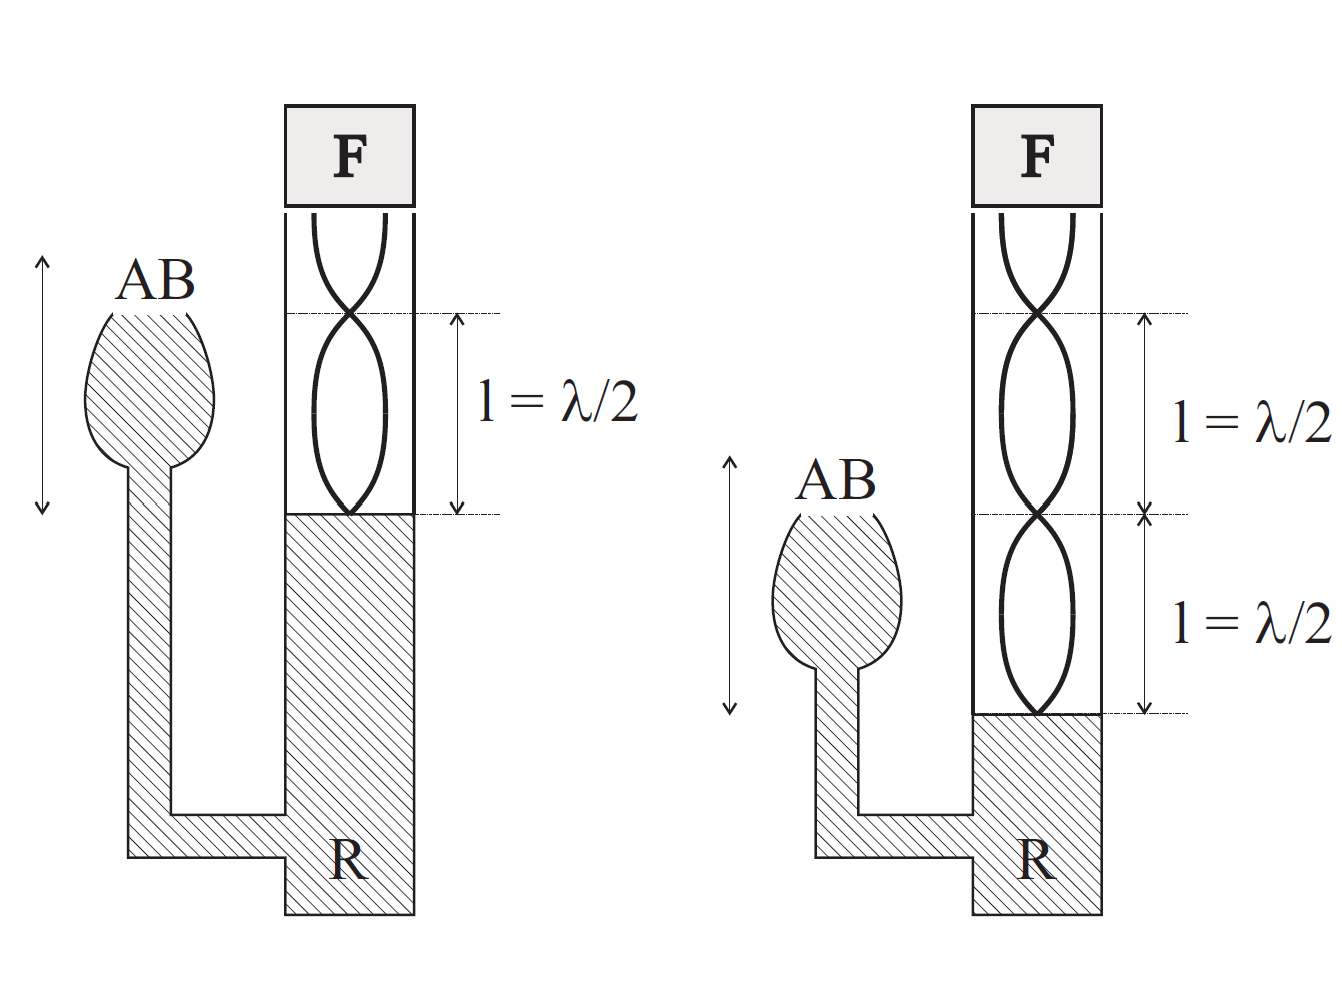
\includegraphics[width=\linewidth]{pics/Fig1.png}
            \caption[Quincke-Resonanzrohr]{Das Quincke-Resonanzrohr. F Frequenzgeber ($\SI[]{1600}{\hertz}$), R Glasrohr mit veränderbarem Wasserspiegel, AB Ausgleichsbehälter, $l$ Länge der
            Luftsäule, $\lambda$ Wellenlänge.}
            \label{fig:Quincke}
        \end{minipage}
        \hspace{.02\linewidth}% Abstand zwischen Bilder
        \begin{minipage}[t]{.51\linewidth} % [b] => Ausrichtung an \caption
            \vspace{-10\baselineskip}
            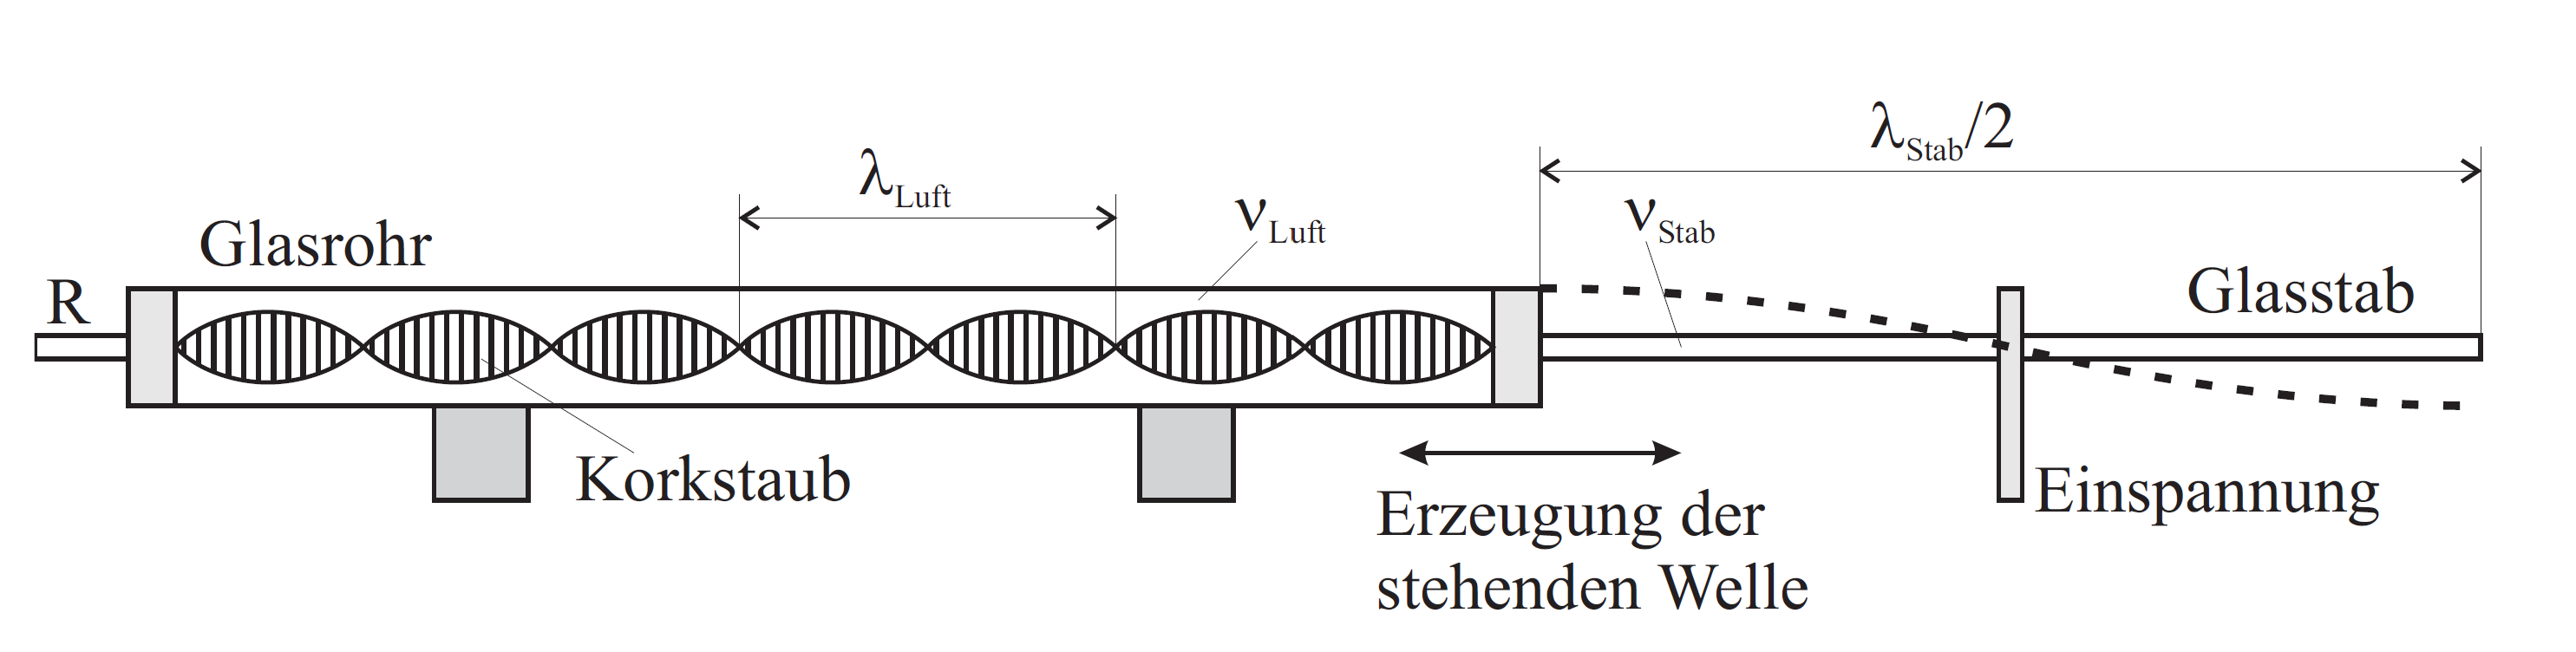
\includegraphics[width=\linewidth]{pics/Fig2.png}
            \caption[Kundt'sches Rohr]{Das Kundt'sche Rohr. $\lambda_{Stab}$, $\lambda_{Luft}$ Wellenlänge im longitudinal schwingenden Glasstab bzw. in der Luft.}
            \label{fig:Kundt}
            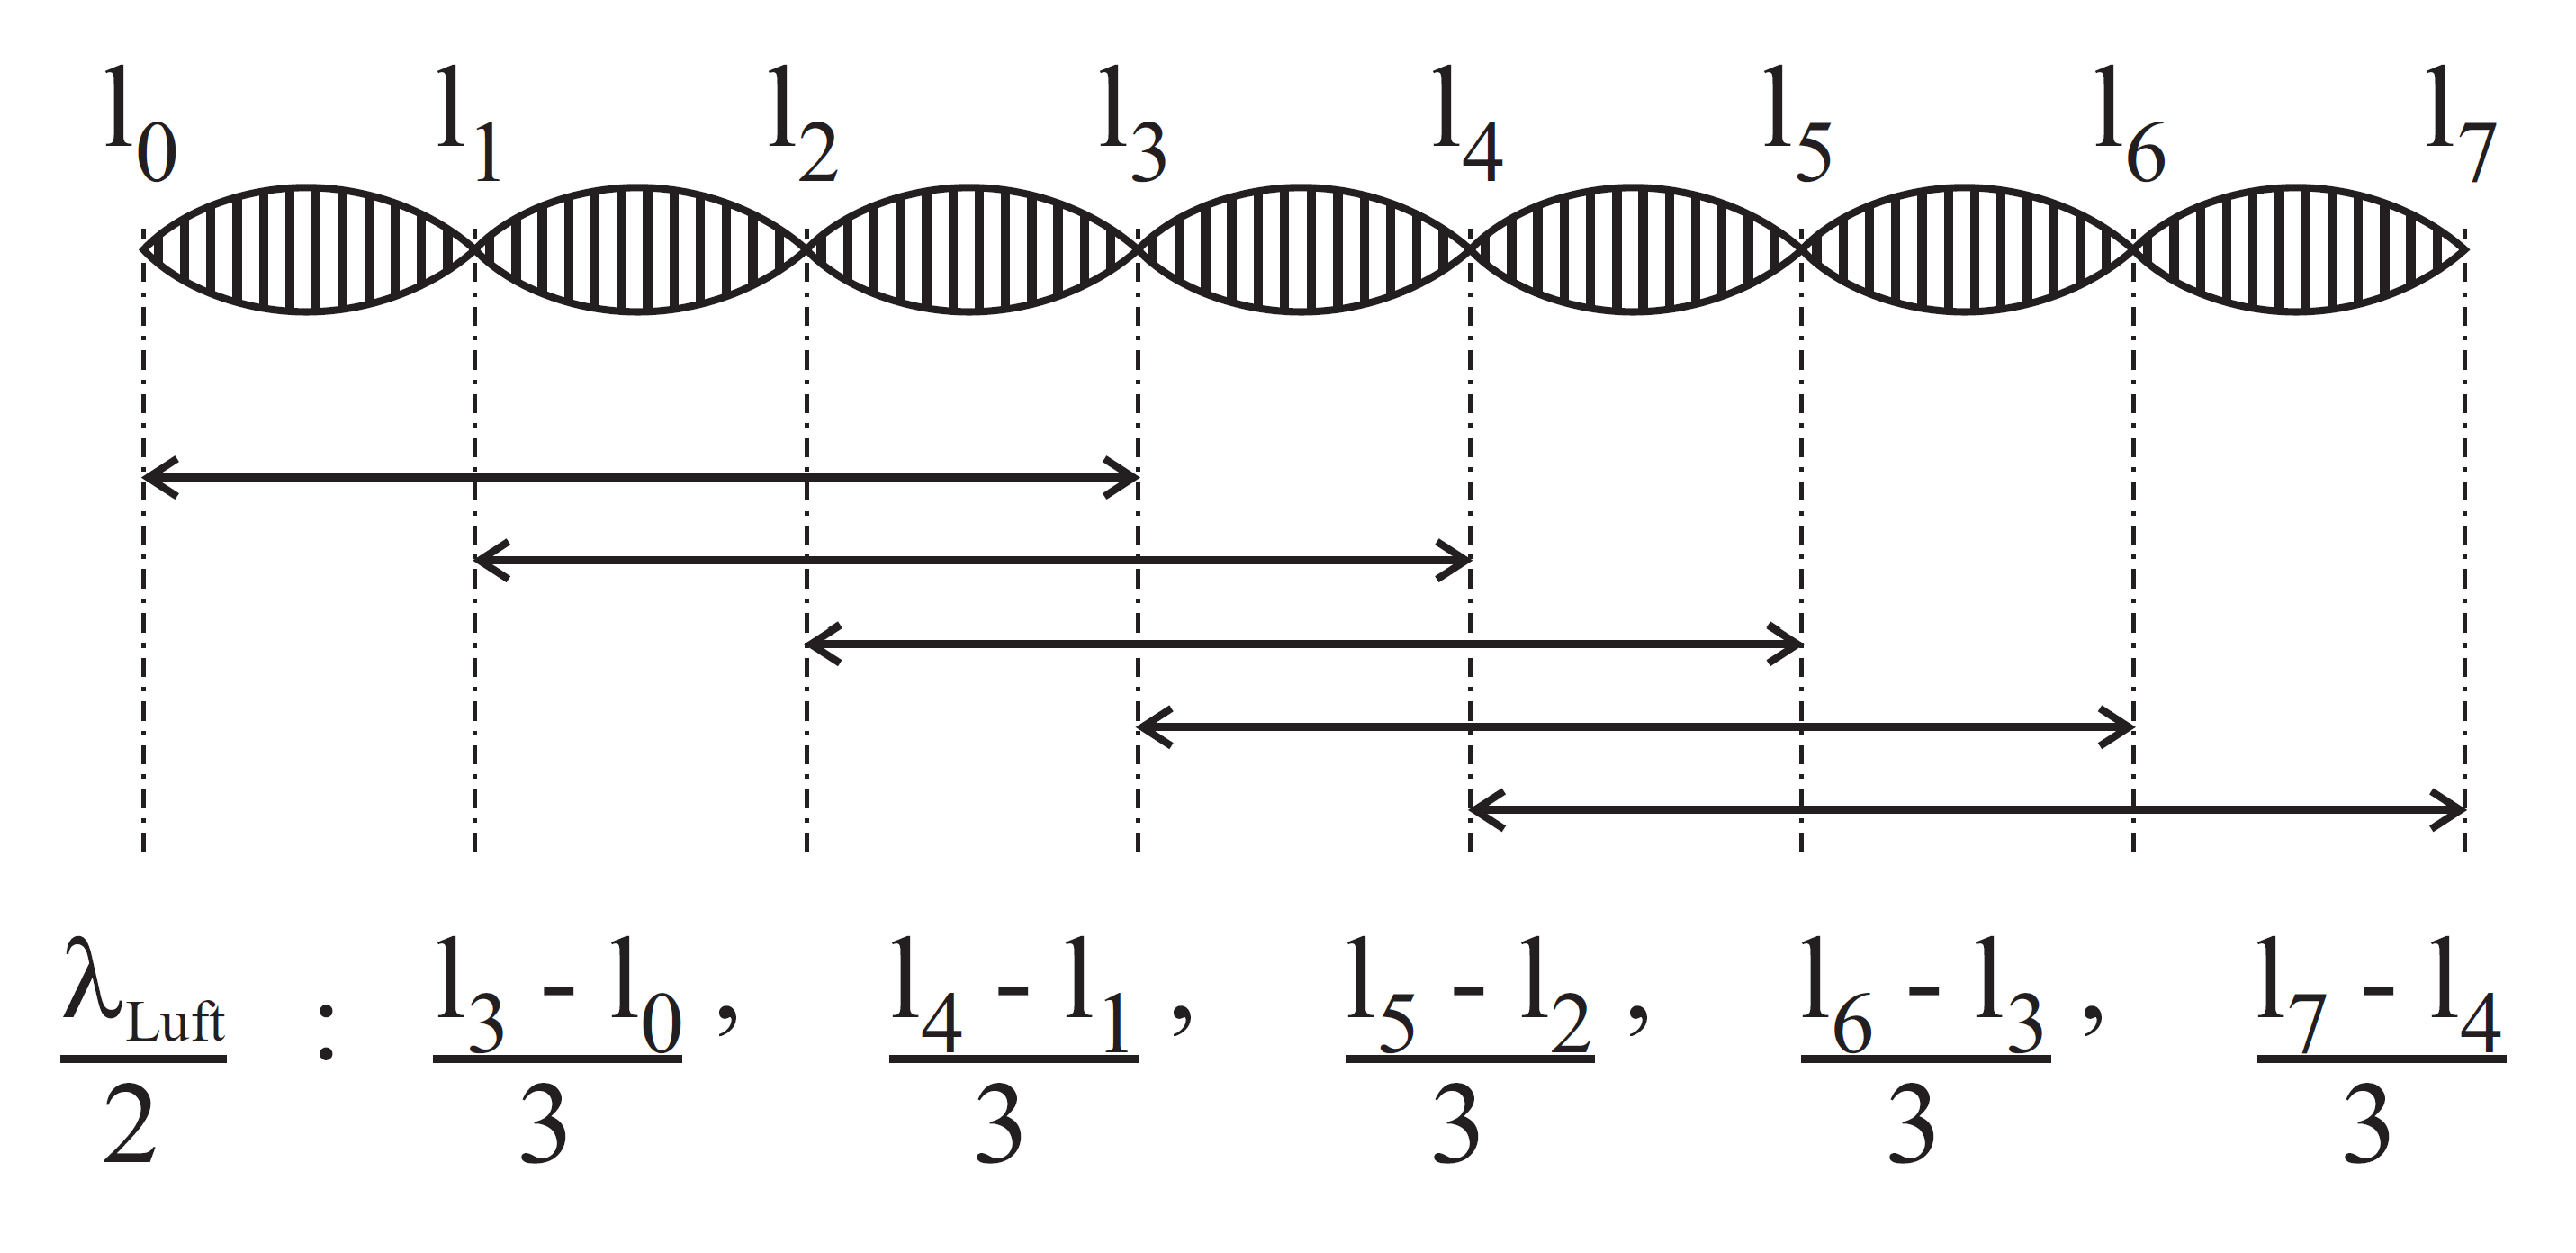
\includegraphics[width=\linewidth]{pics/Fig3.png}
            \caption{Zur Bestimmung der Wellenlänge}
            \label{fig:Wellenlaenge}
        \end{minipage}
    \end{center}
\end{figure}

Zu \autoref{fig:Quincke}: Das Resonanzrohr ist ein Glasrohr, das eine Luftsäule veränderbarer Länge enthält.
Durch Heben und Senken des Ausgleichsbehälters kann man die Länge der Luftsäule variieren.
Die Luftsäule wird durch einen Schallgeber über der Öffnung des Rohres zum Schwingen angeregt.
Die Frequenz ist durch den Schallgeber vorgegeben. Die Wellen laufen bis zum Ende
der Luftsäule (Wasseroberfläche), werden dort reflektiert, und interferieren mit den einfallenden
Wellen, so daß sich im Rohr eine stehende Welle ausbildet. Ist die Luftsäule so lang, daß sich an
der Wasseroberfläche ein Schwingungsknoten, an der Rohröffnung aber ein Schwingungsbauch
befindet, so besteht Resonanz zwischen dem Frequenzgeber und der Luftsäule im Rohr.

Zu \autoref{fig:Kundt}: Die vom Stabende bei longitudinaler Anregung ausgehende Schallwelle pflanzt sich
in das Glasrohr fort, und wird am Ende des Glasrohres reflektiert. Es entsteht eine stehende
Welle, die mittels Korkpulver in der Röhre sichtbar gemacht wird. Die stehende Welle bildet
sich nur dann scharf aus, wenn am geschlossenen Ende des Rohres ein Wellenknoten liegt. Dies
wird erreicht, indem man die Länge der Luftsäule durch Verschieben des Glasrohres variiert.

Zu \autoref{fig:Wellenlaenge}: Zur Bestimmung der Wellenlänge in Luft $\lambda_{Luft}$ werden zunächst alle Knotenstellen
ausgemessen ($l_0,l_1,\dots,l_n$). Soll zur Verbesserung der Ablesefehler der Knotenstellen die
größtmögliche Anzahl von Messungen zur Mittelwertbildung verwendet werden, so werden als
Anfangs- und Endknotenstellen die Knoten herangezogen, deren Abstand voneinander gerade
größer ist als $\frac{a}{2}$, wobei $a$ der Abstand zwischen dem ersten und dem letzten zur Messung
geeigneten Knoten ist. Wie aus \autoref{fig:Wellenlaenge} ersichtlich, ergeben sich dadurch beispielsweise für 6
Meßpunkte 3 voneinander unabhängige Mittelwerte für $\frac{\lambda_{Luft}}{2}$.

\section{Geräteliste}
\label{sec:geraeteliste}
\setlength\LTleft{-6.5em}
\begin{longtable}{c|c|S|p{19em}}
\caption[Geräteliste]{Verwendete Geräte \label{tab:geraeteliste}} \\  % optionales Argument wird in Verzeichnissen verwendet, essentielles Argument direkt im Text
\toprule
Gerät                              & Gerät-Nr. & { Unsicherheit }  & Bemerkungen \\  
\midrule
\endfirsthead
\caption[]{(Fortsetzung)}\\
\toprule
Gerät                              & Gerät-Nr. & { Unsicherheit }  & Bemerkungen \\                                                                        
\midrule
\endhead
\endfoot
\endlastfoot

        Quincke-Resonanzrohr               & axx       & { - }             & Wird verwendet um die Schallgeschwindigkeit zu bestimmen                              \\ \hline
        Maßband                            & bxx       & \SI{1}{\mm}       & Um den Glasstab abzumessen                                                            \\ \hline
        Zollstab                           & cxx       & \SI{1}{\mm}       & Um die Abstände der Knoten bei den stehenden Wellen beim Kundt'schen Rohr zu messen   \\ \hline
        Eisener Zollstab                   & dxx       & \SI{0.5}{\mm}     & Um die Abstände der Knoten bei den Resonanzen im Quincke-Rohr zu bestimmen            \\ \hline
        Flüssigkeit, nicht viskos          & gxx       & { - }             & Zum Befüllen des Quincke-Rohres                                                       \\ \hline
        Signalgenerator                    & hxx       & \SI{0.01}{\hertz} & Sendet einen \SI{1600.00}{\hertz} Sinussignal an den Lautsprecher                     \\ \hline
        Lautsprecher                       & ixx       & { - }             & Zum Anregen von stehenden Wellen im Quincke-Rohr mit der Frequenz vom Signalgenerator \\ \hline
        Thermometer                        & jxx       & \SI{0.6}{\kelvin} & Modell: GTH 1170 (Greisinger GmbH.) Um die Umgebungstemperatur zu bestimmen           \\ \hline
        Kundt'sches Rohr, klein            & kxx       & { - }             & Zur Bestimmung der Frequenz der Trillerpfeie                                          \\ \hline
        Trillerpfeife                      & lxx       & { - }             & -                                                                                     \\ \hline
        Glasstab                           & mxx       & \SI{1500(2)}{\mm} & Zur Anregung von longitudinaler Wellen im Kundt'schen Rohr (groß)                     \\ \hline
        Kundt'sches Rohr, groß             & nxx       & { - }             & Zur Bestimmung des E-Moduls des Glasstabes                                            \\ \hline
        Stoppel                            & oxx       & { - }             & Um sicherzustellen, dass ein Knoten am Ende des Rohres ist                            \\ \hline
        Schwamm                            & pxx       & { - }             & Zum Anregen des Glasstabes                                                            \\ \hline
        Klemmen Halterungen                & qxx       & { - }             & Diverse Befestigungen                                                                 \\ \hline
        Sensor-CASSY \footnote{Die Unsicherheit wurde aus dem Manual des Cassy-Sensors genommen \cite{cassylab}}                       & rxx       & \SI{50}{\um}     & (LD Didactic GmbH) Zum Aufnehmen der Daten des Piezelektr. Körpers                    \\ \hline
        CASSY Lab                          & sxx       & { - }             & (LD Didactic GmbH) Zum Verarbeiten der Daten vom Sensor                               \\ \hline
        Piezoelektr. Körper                & txx       & { - }             & Reagiert auf die Schallwellen im Medium mit einer elektr. Spannung                    \\ \hline
        Stativstange                       & uxx       & \SI{1500(2)}{\mm} & Schützt die Testobjekte                                                               \\ \hline
        Alustange                          & vxx       & \SI{1500(2)}{\mm} & Testobjekt                                                                            \\ \hline
        Messingstange                      & wxx       & \SI{1500(2)}{\mm} & Testobjekt                                                                            \\ \hline
        Kupferstange                       & xxx       & \SI{1500(2)}{\mm} & Testobjekt                                                                            \\ \hline
        Stahlstange                        & yxx       & \SI{1500(2)}{\mm} & Testobjekt                                                                            \\ \hline
        Holzstab                           & zxx       & { - }             & { - }                                                                                 \\ \hline
        PC mit Windows 95/98/NT oder höher & aax       & \SI{1}{\us}       & Um CASSY Lab zu laufen                                                                \\ \hline
        Anregerstab                        & abx       & { - }             & Um die Testobjekte anzuregen                                                          \\ \hline
                                             
        \hline
\end{longtable}

\section{Versuchsdurchführung und Messergebnisse}
\label{sec:versuchsdurchfuehrung_messergebnisse}

Da es drei Objektiven, in diesem Experiment gibt, wird dieses Kapitel
in folgende drei Unterkapitel geteilt:

\begin{enumerate}
    \item \nameref{ssec:Quincke_versuch}
    \item \nameref{ssec:Kundt_versuch}
    \item \nameref{ssec:Stab_versuch}
\end{enumerate}

\subsection{Quincke Resonanzrohr}
\label{ssec:Quincke_versuch}

In den folgenden Punkten wurde der Ablauf des Experiment, beschrieben um
die Wellenlänge $\lambda$ von der Sinusschwingung $\nu=$ \SI{1600.00(1)}{\hertz},
welche durch den Lautsprecher ausgesendet wird. Der Aufbau ist, so
zu vollziehen, wie im Kapitel \nameref{sec:versuchsanordnung} in
\autoref{fig:Quincke} ersichtlich.

\subsubsection{Ablauf}
\begin{enumerate}
    \item Der Ausgleichsbehälter wird so hoch gehoben, dass das Rohr
        fast zur Gänze gefüllt ist.
    \item Nun wird der Ausgleichsbehälter langsam abgesenkt.
    \item Während dem Absenken wird der im Rohr sinkende Wasserspiegel
        mit einer Kamera aufgenommen, wobei ein Zollstab auch neben
        dem Rohr gut ersichtlich zu sehen ist.
    \item Verwendet man ein Videobearbeitungsprogramm kann man
        den genauen Zeitpunkt, der Resonanz bestimmen und somit
        auch das richtige Bild der Aufnahme, welches den Messwert
        beinhaltet.
    \item Das Bild mit dem Messwert wird dann mittels dem Bildbearbeitungsprogramm
        GIMP untersucht. Die maximale Anzahl an sichtbaren Skalenstrichen 
        wurden als Maßstab verwendet um $\pm 7$ px Ableseauflösung zu
        haben.
\end{enumerate}

Durch das mehrmalige Durchführen dieses Ablaufes sind folgende Messwerte
entstanden, siehe \autoref{tab:Quincke_höhenwerte}:

\begin{table}[H]
    \centering
    \caption{Stellen $x_i$ entlang des Zollstabs wo Resonanz im Quinckerohr 
    stattfindet. Alle Messungen sind in \si{\cm} und sind auf \SI{+-0.3}{\mm} }
    \label{tab:Quincke_höhenwerte}
    \begin{tabular}{l|S|S|S|S|S}
        i                     & {Messreihe 1.} & {Messreihe 2.} & {Messreihe 3.} & {Messreihe 4.} & {Messreihe 5.} \\ \hline
        1                     & 3.45           & {-}  & {-}  & {-}  & 3.45 \\
        2                     & 14.25          & 14.15  & 14.10  & 14.15  & 14.15\\
        3                     & 24.95          & 24.95  & 24.65  & 24.90  & 24.90\\
        4                     & 35.55          & 35.60  & 35.60  & 35.40  & 35.40\\
        5                     & 46.30          & 46.25  & 46.30  & 45.90  & 45.90\\
        6                     & 56.75          & 56.75  & 56.90  & 56.95  & 56.95\\ \hline
    \end{tabular}
\end{table}

\subsection{Kundt'sches Rohr}
\label{ssec:Kundt_versuch}

In den folgenden Punkten wurde der Ablauf des Experiment beschrieben um
die Wellenlänge $\lambda$ der stehenden Welle im Kundt'schen Rohr
zu bestimmen.
Der Aufbau ist, so
zu vollziehen, wie im Kapitel \nameref{sec:versuchsanordnung} in
\autoref{fig:Kundt} ersichtlich.

\subsubsection{Ablauf}
\begin{enumerate}
    \item Nachdem Aufbau wird der Glasstab durch einen Schwamm erregt,
        indem dieser entlang des Stabes gezogen wird. 
    \item Dadurch bildet sich eine Welle im Stab, welche an das
        Kundt'sche Rohr weiter gegeben wird.
    \item Die entstandenen stehenden Wellen machen sich durch das Ablagern
        des Korkstaubes im Rohr sichtbar.
    \item Werden die Abstände der Knoten, neben einem Zollstab,
        mit einer Kamera aufgenommen, ist es möglich die Stellen
        der Bäuche zu bestimmen.
    \item Verwendet man ein Videobearbeitungsprogramm kann man
        den genauen Zeitpunkt, der Resonanz bestimmen und somit
        auch das richtige Bild der Aufnahme, welches den Messwert
        beinhaltet.
    \item Das Bild mit dem Messwert wird dann mittels dem Bildbearbeitungsprogramm
        GIMP untersucht. Die maximale Anzahl an sichtbaren Skalenstrichen 
        wurden als Maßstab verwendet um $\pm 15$ px Ableseauflösung zu
        haben.
\end{enumerate}

Durch das Durchführen dieses Ablaufes sind folgende Messwerte
für die Stellen der Knoten entstanden, siehe \autoref{tab:kundt_stellen}:

\begin{table}[H]
    \centering
    \caption{Stellen entlang des Zollstabs wo sich Bäuche der stehenden Wellen
        im Kundt'schen Rohr befinden. Alle Messungen sind in \si{\cm} und sind
    mit einer Unsicherheit von \SI{+-2}{\mm}.}
    \label{tab:kundt_stellen}
    \begin{tabular}{l|S}
        i                     & {Stellen} \\ \hline
    	1                     & 96.9         \\ 
    	2                     & 87.1          \\
    	3                     & 77.0          \\
        4                     & 67.1          \\
        5                     & 57.3          \\
        6                     & 47.2          \\ \hline
    \end{tabular}
\end{table}

\subsection{Schallgeschwindigkeit in Stäben}
\label{ssec:Stab_versuch}

Der Aufbau ist folgender Maßen zu vollziehen. Der, zu untersuchende,
Stab, ist in ein eingespanntes vertikal Rohr einzuführen, damit
dieser frei beweglich bleibt. Am unteren Ende befindet sich ein 
piezoelektrischer Körper, welcher mit dem Cassy Lab System durch
signaltragende Kabel verbunden wird. 
In den folgenden Punkten wurde der Ablauf des Experiment beschrieben um
die Schallgeschwindigkeit $c$ in verschieden Stäben zu bestimmen.

\subsubsection{Ablauf}
\begin{enumerate}
    \item Nachdem Aufbau wird der, zu untersuchende, Stab durch einen
        Schlag angeregt.
    \item Die propagierende Druckwelle wird von dem piezoelektrischen
        Körper in ein Spannungsignal, umgewandelt, welches
        mit dem Cassy Lab aufgezeichnet wird.
    \item Die Daten werden im Cassy Lab mit einer Skala, ausgegeben.
    \item Ein Bild der Messwert wird dann mittels dem Bildbearbeitungsprogramm
        GIMP untersucht. Die maximale Anzahl an sichtbaren Skalenstrichen 
        wurden als Maßstab verwendet um $\pm 4$ px Ableseauflösung zu
        haben.
\end{enumerate}

Durch das Durchführen dieses Ablaufes sind folgende Messwerte
für die Abstände von $n$ Perioden entstanden, siehe \autoref{tab:Stab_pixel}:

\begin{table}[H]
    \centering
    \caption{Den gemessenen Abstand $l$ (in \si{\px}) von $n$ Perioden 
        mit einem Maß $m$ (in \si{\px\per5\ms}), welches Pixel in Zeit
        umwandelt. Alle $l$ Werte haben eine Unsicherheit von \SI{4}{\px} und
        $m$ Werte haben eine Unsicherheit von \SI{4}{\px\per5\ms}. Diese drei Werte
        wurden für folgende Stoffe aus
        den Diagrammen ermittelt. \\
    $l_A$, $n_A$, $m_A$ sind die drei zuvor erwähnten Werte für Aluminium\\
    $l_K$, $n_K$, $m_K$ sind die drei zuvor erwähnten Werte für Kupfer\\
    $l_M$, $n_M$, $m_M$ sind die drei zuvor erwähnten Werte für Messing\\
    $l_S$, $n_S$, $m_S$ sind die drei zuvor erwähnten Werte für Stahl\\
    }
    \label{tab:Stab_pixel}
    \hspace*{-1.5cm}
    \begin{tabular}{l|S[table-format=1.0(0)]|S[table-format=4.0(0)]|S[table-format=4.0(0)]|S[table-format=1.0(0)]|S[table-format=4.0(0)]|S[table-format=4.0(0)]|S[table-format=1.0(0)]|S[table-format=4.0(0)]|S[table-format=4.0(0)]|S[table-format=1.0(0)]|S[table-format=4.0(0)]|S[table-format=4.0(0)]}
        i  & $n_A$ & $l_A$ & $m_A$ & $n_K$ & $l_K$ & $m_K$ & $n_M$ & $l_M$ & $m_M$ & $n_S$ & $l_S$ & $m_S$ \\ \hline 
        {Einheit}  & {-}     & \si{\px}  & \si{\px\per5\ms}  & {-}     & \si{\px}   & \si{\px\per5\ms}  & {-}     & \si{\px}   & \si{\px\per5\ms}  & {-}     & \si{\px}  & \si{\px\per5\ms}  \\ \hline
        1  & 9     & 1222  & 1263  & 6     & 996   & 1254  & 5     & 860   & 1270  & 9     & 1206  & 1248  \\ \hline
        2  & 9     & 1182  & 1262  & 6     & 992   & 1258  & 6     & 1084  & 1270  & 9     & 1199  & 1247  \\ \hline
        3  & 9     & 1165  & 1261  & 6     & 990   & 1256  & 6     & 1067  & 1271  & 9     & 1205  & 1246  \\ \hline
        4  & 8     & 1055  & 1260  & 7     & 1190  & 1260  & 4     & 642   & 1271  & 9     & 1206  & 1246  \\ \hline
        5  & 9     & 1206  & 1258  & 7     & 1191  & 1256  & 5     & 869   & 1276  & 9     & 1208  & 1248  \\ \hline
        6  & 9     & 1213  & 1258  & 7     & 1187  & 1256  & 5     & 869   & 1272  & 9     & 1206  & 1249  \\ \hline
        7  & 9     & 1157  & 1264  & 7     & 1192  & 1253  & 5     & 870   & 1275  & 9     & 1206  & 1248  \\ \hline
        8  & 9     & 1197  & 1260  & 6     & 991   & 1254  & 5     & 872   & 1275  & 8     & 1056  & 1246  \\ \hline
        9  & 8     & 1057  & 1258  & 7     & 1190  & 1262  & 4     & 642   & 1270  & 8     & 1055  & 1250  \\ \hline
        10 & 8     & 1054  & 1258  & 7     & 1191  & 1262  & 5     & 869   & 1270  & 8     & 1059  & 1250  \\ \hline
        11 & {-}   & {-}  & {-} & 6     & 991   & 1252  & {-}   & {-}   & {-}      & {-}   & {-}   & {-} \\ \hline
    \end{tabular}
\end{table}


\section{Auswertung}
\label{sec:auswertung}

Da es drei Objektiven, in diesem Experiment gibt, wird dieses Kapitel
in folgende drei Unterkapitel geteilt:

\begin{enumerate}
    \item \nameref{ssec:Quincke_auswertung}
    \item \nameref{ssec:Kundt_auswertung}
    \item \nameref{ssec:Stab_auswertung}
\end{enumerate}

\subsection{Quincke-Resonanzrohr Auswertung}
\label{ssec:Quincke_auswertung}
Kombiniert man nun die Messwerte aus dem Kapitel \nameref{ssec:Quincke_versuch} 
mit den Gleichungen aus \nameref{sec:voraussetzungen_grundlagen}
kommt man zuerst auf die mehrere Messwerte für die Wellenlänge $\lambda$
der Schallwelle und kombiniert mit der Frequenz $\nu$ des Signalgenerators
kann die Schallgeschwindigkeit in Luft $c_{Luft}$, nach \autoref{eq:cist},
bestimmt werden.

\begin{table}[H]
    \centering
    \caption{Errechnete Wellenlängen $\lambda_i = x_{i+1}-x_{i}$ (in \si{\cm})
        aus den Daten, der \autoref{tab:Quincke_höhenwerte},
        von einer Sinusschwingung mit \SI{1600.00(1)}{\hertz}. Wobei $\lambda$
        der Mittelwerte der Messwerte $\lambda_i$ ist und der Fehler den 
        Standarderror und den Fehler bei der
        Manufaktur des Zollstabs (ein Skalenabstand auf die Gesamtlänge 
        also \SI{+-0.5}{\mm}) berücksichtig.}
    \label{tab:quincke_lambda}
    \begin{tabular}{r|S|S|S|S|S}
        i & {Messreihe 1.} & {Messreihe 2.} & {Messreihe 3.} & {Messreihe 4.} & {Messreihe 5.} \\ \hline
        1 & 10,8           & { - }               &  { - }              &   { - }             & 10,75  \\ 
        2 & 10,7           & 10,8           & 10,55          & 10,75          & 10,8   \\ 
        3 & 10,6           & 10,65          & 10,95          & 10,5           & 10,75  \\ 
        4 & 10,75          & 10,65          & 10,7           & 10,5           & 10,75  \\ 
        5 & 10,45          & 10,5           & 10,6           & 11,05          & 10,5   \\ \hline \hline
        $\lambda$ & \SI{10.68(9)}{\cm} & & & & \\
    \end{tabular}
\end{table}

Mit $\lambda$ und $\nu$ bekannt erhält man 
für die Schallgeschwindigkeit in Luft:

\begin{equation*}
    c_{Luft}= \SI{342(3)}{\meter\per\second}
\end{equation*}

Da $c_{Luft}$ nun bekannt ist, ist es für uns auch möglich die Adiabatenexponente
$\kappa$ mit der Umgebungstemperatur $\theta =$ \SI{18.4(6)}{\celsius}, wenn 
\autoref{eq:kappa_c} nach $\kappa$ umformt wird, zu bestimmen. Zudem
wurden $p_0 =$ \SI{1013.25}{\hecto\pascal} \cite{Demtroeder2006}
und $\rho_0=$ \SI{1.29e-3}{\gram\per\cm\cubed} \cite{QuinckeKundt2012}
von diesen Quellen entnommen. Man kommt somit
auf einen Wert von \num{1.39(3)} für $\kappa$.

\subsection{Kundt'sches Rohr Auswertung}
\label{ssec:Kundt_auswertung}
Kombiniert man nun die Messwerte aus dem Kapitel \nameref{ssec:Kundt_versuch} 
mit den Gleichungen aus \nameref{sec:voraussetzungen_grundlagen}
kommt man zuerst auf die mehrere Messwerte für die Wellenlänge $\lambda$
mit \autoref{eq:lambda_avg} indem man über Messpunkte, die über einen Abstand
von \num{1.5} Wellenlängen spannen, gemittelt
wird $\lambda_i=\frac{2(l_{i+2}-l_{i})}{3}$. 

\begin{table}[H]
    \centering
    \caption{Errechnete Wellenlängen $\lambda_i=\frac{2(l_{i+2}-l_{i})}{3}$(in \si{\cm})
        aus den Daten, der \autoref{tab:kundt_stellen}, von einer
        im Kundt'schen Rohr entstanden stehende Welle. Wobei $\lambda$
        der Mittelwerte der Messwerte $\lambda_i$ ist und der Fehler den 
        Standarderror und den Fehler bei der
        Manufaktur des Zollstabs (ein Skalenabstand auf die Gesamtlänge 
        also \SI{+-1}{\mm}) berücksichtig.}
    \label{tab:kundt_lambda}
    \begin{tabular}{r|S}
        i & {$\lambda_i$} \\ \hline
        1 & 19.87         \\ 
        2 & 19.87         \\ 
        3 & 19.87         \\ \hline \hline
        $\lambda$ & \SI{19.9(2)}{\cm}\\
    \end{tabular}
\end{table}

Da man durch diese Methode dreimal die gleiche Zahl für die Daten
bekommen hat, wurden die Werte um einen Millimeter variiert und die
maximale Abweichung bestimmt und dieser dem Herstellerfehler 
hinzufügt und aufgerundet.

Mit der Wellenlänge $\lambda_{Luft}=\SI{19.9(2)}{\cm}$ und der in
\nameref{ssec:Quincke_auswertung} gemessenen Schallgeschwindigkeit
$c_{Luft}$ ist es möglich anhand \autoref{eq:wellenlangen_verhaltnis}
die Schallgeschwindigkeit im Glasstab $c_{Glas}$ zu bestimmen. Da die
Wellenlänge im Glas $\lambda_{Glas} = \SI{300.0(4)}{\cm}$,
wie in \autoref{fig:Kundt} 
ersichtlich, die doppelte Länge des Glasstabes, siehe 
\autoref{tab:geraeteliste} mxx, ist. Somit bekommt man einen Wert
für die Schallgeschwindigkeit in Glas: 

\begin{equation*}
    c_{Glas}=\SI{5160(100)}{\meter\per\second}
\end{equation*}

Weiters lässt sich mit der Dichte von Glass $\rho_{Glas}=\SI{2500}{\kg\per\meter\cubed}$ \cite{glassdichte}
durch \autoref{eq:stab_E} der E-Modul des
Glasstabes bestimmen:

\begin{equation*}
    E_{Glas} = \SI{67(3)}{\GPa} 
\end{equation*}

\subsection{Bestimmung des E-Moduls von diversen Materialien}
\label{ssec:Stab_auswertung}
Nimmt man nun die Messwerte aus dem Kapitel \nameref{ssec:Stab_versuch}
ist es möglich die Schallgeschwindigkeiten $c$ in den diversen Materialien
zu bestimmen, folgender einfachen Beziehung:

\begin{equation*}
    c = \frac{2L}{t}
\end{equation*}

Wobei $L$ die Länge des Stabes ist und $t$ die Periodendauer des
aufgenommen Signals ist. $t$ lässt sich mit den Daten aus \autoref{tab:Stab_pixel}
wie folgt berechnen:

\begin{equation}
    t_{*_i} = \frac{5l_{*_i}}{m_{*_i}} \label{eq:relationtimetoobservable}
\end{equation}

Wobei $*$ ein Platzhalter für die diveresen Material Initialien ist.
Mit dieser \autoref{eq:relationtimetoobservable} erhalten
wir folgende Messwerte für die Peridendauern $t_{*_i}$:

\begin{table}[H]
    \centering
    \caption{Errechnete Periodendauern $t_{*_i} = \frac{5l_{*_i}}{m_{*_i}}$(in \si{\ms})
        aus den Daten, der \autoref{tab:Stab_pixel}, von einer
        im durch Anschlagen im Stab enstandene propagierende Welle. 
        Wobei $t_{*}$ der Mittelwerte der Messwerte 
        $t_{*_i}$ von dem Material $*$ ist und der Fehler den 
        Standarderror und das maximale Auflöseverfögen
        einer RS-232 Verbindung ($\SI{+-50}{\us}$) berücksichtigt. \\
        $t_{A_i}$, $t_A$ sind die gemessenen Periodendauern und deren Mittelwerte für Aluminium\\
        $t_{K_i}$, $t_K$ sind die gemessenen Periodendauern und deren Mittelwerte für Kupfer\\
        $t_{M_i}$, $t_M$ sind die gemessenen Periodendauern und deren Mittelwerte für Messing\\
    $t_{S_i}$, $t_S$ sind die gemessenen Periodendauern und deren Mittelwerte für Stahl\\}
    \label{tab:Stab_times}
    \begin{tabular}{r|S[table-format=1.3(3)]|S[table-format=1.3(3)]|S[table-format=1.3(3)]|S[table-format=1.3(3)]}
        i  & {$t_{A_i}$} & {$t_{K_i}$} & {$t_{M_i}$} & {$t_{S_i}$} \\ \hline
       1  & 0,605     & 0,794     & 0,846     & 0,604     \\
       2  & 0,585     & 0,789     & 0,854     & 0,601     \\
       3  & 0,577     & 0,788     & 0,839     & 0,604     \\
       4  & 0,598     & 0,787     & 0,842     & 0,605     \\
       5  & 0,599     & 0,790     & 0,851     & 0,605     \\
       6  & 0,603     & 0,788     & 0,854     & 0,603     \\
       7  & 0,572     & 0,793     & 0,853     & 0,604     \\
       8  & 0,594     & 0,790     & 0,855     & 0,605     \\
       9  & 0,600     & 0,786     & 0,843     & 0,603     \\
       10 & 0,598     & 0,786     & 0,855     & 0,605     \\
       11 & {-}       & 0,792     & {-}       & {-}       \\ \hline \hline
       -  & {$t_{A}$}   & {$t_{K}$}   & {$t_{M}$}   & {$t_{S}$}   \\ \hline
       -  & 0,593(17) & 0,789(11)  & 0,849(16)  & 0,604(10)  \\ \hline \hline
    \end{tabular}
\end{table}

Um die maximale zeitliche Unsicherheit zu bestimmen
wurde Angenommen das jede zeitlich Messung plus minus ein Packet genau
bestimmt wurde und da der Standard RS-232 verwendet wurde kommt man
auf eine zeitliche Unsicherheit von \SI{+-50}{\us}. Da jedoch immer mehrer
Perioden gemessen wurde, verkleinert sich diese Unsicherheit um den
Mittel der Anzahl der Perioden.
Weiters erhält man die folgenden Werte für die Schallgeschwindigkeiten:

\begin{table}[H]
    \centering
    \caption{Schallgeschwindigkeiten in diverser Materialien:\\
    $c_A$ Schallgeschwindigkeit in Aluminium \\
    $c_K$ Schallgeschwindigkeit in Kupfer \\
    $c_M$ Schallgeschwindigkeit in Messing \\
    $c_S$ Schallgeschwindigkeit in Stahl \\
    Alle Werte haben die Einheit \si{\meter\per\second}}
    \label{tab:schallgeschwindigkeiten}
    \begin{tabular}{c|S[table-format=4.0(0)]|S[table-format=4.0(0)]}
        {}    & {Wert} & {$\Delta$} \\ \hline
        $c_A$ & 5060 & +-150   \\
        $c_K$ & 3800 & +-60  \\
        $c_M$ & 3530 & +-80  \\
        $c_S$ & 4970 & +-70  \\
    \end{tabular}
\end{table}

Durch \autoref{eq:stab_E} lässt sich wie bei \nameref{ssec:Kundt_auswertung}
das E-Modul der diversen Materialien bestimmen:

\begin{table}[H]
    \centering
    \caption{E-Module von diverser Materialien berechnet durch
        mit den Schallgeschwindigkeiten $c_*$ aus \autoref{tab:schallgeschwindigkeiten}
        und den Dichten $\rho_*$ der Materialien $*$:\\
    $E_A$ E-Modul und die Dichte $E_A$ von Aluminium \\
    $E_K$ E-Modul und die Dichte $E_K$ von Kupfer \\
    $E_M$ E-Modul und die Dichte $E_M$ von Messing \\
    $E_S$ E-Modul und die Dichte $E_S$ von Stahl \\}
    \label{tab:label}
    \begin{tabular}{c|S|S|S}
        Materialien & {$E_* / \si{\GPa}$} & {$\Delta E_* / \si{\GPa}$} & {$\rho_* / \si{\kg\per\meter\cubed}$}\\
        $Aluminium$ & 69                  & +-5           & 2700 \\
        $Kupfer$    & 130                 & +-4           & 8960 \\
        $Messing$   & 109                 & +-5           & 8730 \\
        $Stahl$     & 190                 & +-6           & 7850 \\
    \end{tabular}
\end{table}

\section{Zusatz am Genfer See}
Als Zusatzaufgabe soll sich ein Verfahren überlegt werden, wie man vor 200
Jahren in der Schweiz die Schallgeschwindigkeit von Wasser bestimmen hätte
können.

Um dies zu vollbringen, läutet eine Person auf der einen Seite des Sees mit der
Glocke unter Wasser, um ein Signal auszusenden. Gleichzeitig wird ein
Lichtblitz ausgesandt, um die Zeitmessung auf der anderen Seite zu starten. Mit
einem Hörrohr wird nun auf der anderen Seite auf das akustische Signal gewartet
und so über Laufzeitmessung die Geschwindigkeit des Signals errechnet. Dazu
muss natürlich die Distanz der beiden Uferseiten bekannt sein.

\section{Diskussion und Zusammenfassung}
\label{sec:diskussion_zusammenfassung}
% Aufzählung was scheiße glaufen is

Nun werden die verwendeten Methoden diskutiert und die Ergebnisse 
zusammengefasst.

\subsection{Diskussion}
Bei der Bestimmung der Schallgeschwindigkeit beim
\nameref{ssec:Quincke_versuch} sind dankt der hinzufügten Tonspur und der
Aufzeichnung die Resonanzstellen sehr gut bestimmbar. Dadurch konnte die
Schallgeschwindigkeit mit kleinen Fehlerbalken relativ zum errechnten Wert
bestimmt werden.  Der erhaltne Wert für die Schallgeschwindigkeit beinhaltet in
seiner Unsicherheit, dennoch den Literaturwert, siehe \autoref{tab:ergebnisse}.
Weiters wurde noch die Adiabatenexponente $\kappa$ bestimmt, welche auch, wegen
den niedrigen Unsicherheiten der Schallgeschwindigkeit, eine niedrige relative
Unsicherheit besitzt. Der erhaltene Wert beinhaltet in seiner Unsicherheit auch
den Literaturwert, siehe \autoref{tab:ergebnisse}.

Bei der Bestimmung des E-Modul $E_{Glas}$ eines Glasstabes wurde ein
Kundt'sches Rohr verwendet um zunächst die Schallgeschwindigkeit $c_{Glas}$ im
Stab zu bestimmen.  Durch die Bestimmung der Stellen der Bäuche mittels
Bildbearbeitungsprogramm und der, in \nameref{sec:versuchsanordnung} erwähnten,
Messwertmittelung konnte die Wellenlänge von einer stehenden Welle bestimmt
werden. Durch die die Schallgeschwindigkeit $c_{Glas}$ und auch gleich der
E-Modul $E_{Glas}$ bestimmt wurde. Die Werte beinhalten die Literaturwerte in
ihrer Unsicherheit, siehe \autoref{tab:ergebnisse}.

Bei der Bestimmung der E-Module der diversen Materialien konnte die Länge und
Zeit wieder genau bestimmt werden durch die Verwendung eines
Bildbearbeitungsprogramm. Dadurch sind selbst die relative Unsicherheiten der
dreifachen Standardabweichung niedrig, der Schallgeschwindigkeit und der
E-Module in den diversen Materialien. Alle erhaltenen Werte beinhalten die
Literaturwerte in ihren Unsicherheitsintervallen, siehe
\autoref{tab:ergebnisse}.

\begin{table}[H]
    \centering
    \caption{Hier werden die erhaltenen Werte den Literaturwerten gegenübergestellt.\\
    $c_{Luft}$ die Schallgeschwindigkeit in Luft \\ 
    $\kappa$ die Adiabatenexponente von Luft \\
    $E_{Glas}$ E-Modul von und die Schallgeschwindigkeit $c_{Glas}$ in Glas \\
    $E_A$ E-Modul von und die Schallgeschwindigkeit $c_A$ in Aluminium \\
    $E_K$ E-Modul von und die Schallgeschwindigkeit $c_K$ in Kupfer \\
    $E_M$ E-Modul von und die Schallgeschwindigkeit $c_M$ in Messing \\
    $E_S$ E-Modul von und die Schallgeschwindigkeit $c_S$ in Stahl \\
    Alle Werte wurden unter folgenden Bedingungen aufgenommen: \\
    Umgebungstemperatur @ \SI{18.4(6)}{\celsius} \\
    Luftdruck @ \SI{1013.25}{\hecto\pascal} \\ 
    Luftdichte @ \SI{1.29e-3}{\gram\per\cm\cubed} \\}
    \label{tab:ergebnisse}
    \begin{tabular}{c|S|S}
        Symbol:    & {Bestimmter Wert}                  & {Literaturwert}           \\ \hline
        $c_{Luft}$ & \SI{342(3)}{\meter\per\second}     & \SI{343.2}{\meter\per\second} \cite{schallvelocity}    \\
        $\kappa$   & \num{1.39(3)}                      & \num{1.417} \cite{ahrberg2011handbuch}  \\
        $c_{Glas}$ & \SI{5.16(10)e3}{\meter\per\second} & \SI{5.14e3}{\meter\per\second} \cite{extensionalspeedofsound}     \\
        $E_{Glas}$ & \SI{67(3)}{\GPa}                   & \SIrange{50}{90}{\GPa} \cite{youngallengineering}   \\
        $c_A$      & \SI{5.06(15)e3}{\meter\per\second} & \SI{5.00e3}{\meter\per\second} \cite{extensionalspeedofsound}   \\
        $c_K$      & \SI{3.80(6)e3}{\meter\per\second}  & \SI{3.81e3}{\meter\per\second} \cite{extensionalspeedofsound}   \\
        $c_M$      & \SI{3.53(8)e3}{\meter\per\second}  & \SI{3.48e3}{\meter\per\second} \cite{extensionalspeedofsound}   \\
        $c_S$      & \SI{4.97(7)e3}{\meter\per\second}  & \SI{5.00e3}{\meter\per\second} \cite{extensionalspeedofsound}   \\
        $E_A$      & \SI{69(5)}{\GPa}                   & \SI{68.9}{\GPa} \cite{youngaluminium} \cite{youngaluminiumextra} \\
        $E_K$      & \SI{130(4)}{\GPa}                  & \SIrange{121}{138}{\GPa} \cite{armstrong2009measuring}\\
        $E_M$      & \SI{109(5)}{\GPa}                  & \SIrange{102}{125}{\GPa} \cite{youngallengineering} \\
        $E_S$      & \SI{190(6)}{\GPa}                  & \SI{193}{\GPa} \cite{youngrolledstainlesssteel} \\
    \end{tabular}
\end{table}

\subsection{Zusammenfassung}

Da alle erhaltenen Werte die Literaturwerte beinhalten lässt sich sagen
dass die Methoden zureichend sind um diese Werte zu bestimmen. Wenn
die Auswertung richtig gemacht wurde sind auch die relativen Unsicherheiten
aller Werte niedrig. Im Ganzen lässt sich sagen dass dieses Experiment
die Literaturwerte weiter unterstützt. 

Ein Vebesserungs Vorschlag wäre, wenn die Werte noch genauer bestimmt werden
müssen genauer Messgeräte verwendet werden. Außer beim Kundt'schen Rohr
dort müssen sollte man vielleicht die Glasstange mehrmals anregen und
noch mehr Messwerte sammeln.

% Literaturtabelle
\newpage
\printbibliography

\listoffigures

\listoftables


\end{document}
